% TEXINPUTS=.:$HOME/git/bvtex: latexmk  -pdf <main>.tex
\documentclass[xcolor=dvipsnames]{beamer}

\input{defaults}
\input{beamer/preamble}

\setbeamertemplate{navigation symbols}{}
% \setbeamertemplate{background}[grid][step=1cm]

\usepackage{siunitx}
\usepackage{xmpmulti}
\usepackage[export]{adjustbox}

\usepackage[outline]{contour}
\usepackage{tikz}
\usetikzlibrary{shapes.geometric, arrows}
\usetikzlibrary{positioning}

\definecolor{bvtitlecolor}{rgb}{0.98, 0.92, 0.84}
\definecolor{bvoutline}{rgb}{0.1, 0.1, 0.1}

\renewcommand{\bvtitleauthor}{Brett Viren\\\small for the BNL Wire Cell Group}
\renewcommand{\bvtit}{Wire Cell}
\renewcommand{\bvtitle}{\LARGE Wire Cell Event Reconstruction Software
for LArTPC Detectors}
\renewcommand{\bvevent}{BNL CSC Seminar 2015 Sep 29}
\renewcommand{\bvbeamerbackground}{}

% http://tex.stackexchange.com/a/23550
\makeatletter
\providecommand{\beamer@slideinframe}{0}%
\tikzset{highlight/.code={\ifnum#1=\beamer@slideinframe \tikzset{draw=red,text=red}\fi},highlight/.value required}
\makeatother

\setbeamertemplate{headline}{%
\leavevmode%
  \hbox{%
    \begin{beamercolorbox}[wd=\paperwidth,ht=2.5ex,dp=1.125ex]{palette quaternary}%
    \insertsectionnavigationhorizontal{\paperwidth}{}{\hskip0pt plus1filll}
    \end{beamercolorbox}%
  }
}
\begin{document}
\input{beamer/title.tex}
\input{beamer/toc.tex}

\lstset{%
  language=C++,
                basicstyle=\scriptsize\ttfamily,
                keywordstyle=\color{blue}\ttfamily,
                stringstyle=\color{red}\ttfamily,
                commentstyle=\color{gray}\ttfamily,
                morecomment=[l][\color{magenta}]{\#}
}

\section {Physics Context}

\begin{frame}
  \frametitle{}
  
\end{frame}

\begin{frame}
  \frametitle{LArTPC Experiments - Icarus}

  \begin{columns}
    \begin{column}{0.5\textwidth}
      \begin{itemize}
      \item Two \SI{300}{\tonne} modules in Gran Sasso tunnel, Italy.
      \item Took data from CERN neutrino beam.
      \item Moving to Fermilab for short-baseline neutrino program.
      \end{itemize}
    \end{column}
    \begin{column}{0.5\textwidth}
      \includegraphics[width=0.8\textwidth]{icarus.png}
    \end{column}
  \end{columns}
\end{frame}

\begin{frame}
  \frametitle{LArTPC Experiments - MicroBoone}

  \begin{columns}
    \begin{column}{0.5\textwidth}
      \begin{center}
        \includegraphics[width=0.9\textwidth]{run1148_ev1016.png}
      \end{center}

    \end{column}
    \begin{column}{0.5\textwidth}
      \begin{itemize}
      \item \SI{85}{\tonne} fiducial mass.
      \item 8256 channels
      \item 3 mm wire pitch.
      \item Investigate LSND-effect, look for sterile-$\nu$, $\nu$-Ar
        cross sections.
      \end{itemize}
    \end{column}
  \end{columns}

  \begin{center}
    Just started taking data at Fermilab!    
  \end{center}

\end{frame}

\begin{frame}[fragile]
  \frametitle{LArTPC Experiments - 
\includegraphics[height=7mm,trim=4cm 9.2cm 4cm 9.3cm,clip,valign=c]{DUNElogo_colorHORIZONTAL.pdf}}
  \begin{itemize}\footnotesize
  \item \SI{35}{\tonne} prototype (at FNAL) commissioning now, running early 2016.
  \item Full-scale ``protoDUNE'' (at CERN) 2017 with $\pi, K, p$ beam tests.
  \item Full far detector to be underground in South Dakota $\sim$2025.
    \begin{itemize}
    \item \SI{40}{\kilo\tonne} fiducial mass in 4 modules.
    \item 5 mm wire pitch, 1.5M channels.
    \item \textbf{CP-violation, proton decay, supernovae neutrino bursts}.
    \end{itemize}
  \item Underground construction forces added complication of wrapped
    induction wires and two sided anode planes.
  \end{itemize}

  \begin{center}
    \includegraphics[height=3cm]{LBNF_Graphic_021715-1024x340.png}
  \end{center}

\end{frame}

\begin{frame}[fragile]
  LArTPC = \textbf{L}iquid \textbf{Ar}gon \textbf{T}ime \textbf{P}roportional \textbf{C}hamber

  \begin{center}
      \transduration<0-16>{0}
      \multiinclude[<+->][format=png, graphics={height=0.7\textheight}]{signal}
  \end{center}

  \begin{minipage}[t][1cm]{1.0\textwidth}
    \only<1>{Charged particles traverse the detector at relativistic
      speeds and leave behind ionized Argon.}

    \only<2>{Ion and electron pairs drift off in opposite directions
      in the E-field applied between anode wires and cathode plane.}

    \only<3>{Here we watch the electrons drift.
      They drift with a speed of
      \SI{1.6}{\milli\meter\per\micro\second} toward the anode wire planes.}

    \only<4>{As they approach, they begin to induce signals on the
      nearby wires.}

    \only<5>{There are two planes of induction wires which see a
      bipolar signal as charge drifts by.}

    \only<6>{The final plane collects the drifting charge and thus sees a unipolar signal.}

    \only<7>{The exact signal response is complicated and depends on
      details of the electric field and detector construction.}

    \only<8>{Charge on each wire is digitized as a function of time.
      Typical digitization ``tick'' is
      \SI{0.5}{\micro\second}, wire spacing is \num{3} to \SI{5}{\milli\meter}.}

    \only<9>{Measuring the drifted charge requires a deconvolution of a
      response function and a noise filter with the raw wire signals.}

    \only<10>{As a batch of electrons drift, it diffuses out in both
      the longitudinal and transverse directions. LAr impurities cause
      attenuation.} 

    \only<11>{At the maximum drift distance allowed by the
      detector, diffusion can be as much as \SI{1}{\micro\second}
      longitudinally and \SI{2.5}{\milli\meter} transverse.} 

    
    \only<12>{Still drifting...} 
    
    \only<13>{Still drifting...
    It's a slow detector!}
    
    \only<14>{Still drifting...} 

    \only<15>{Each wire plane reads out one 2D view (wire pitch
      direction vs. time) of the drifting charge pattern.}
    
    \only<16>{Combining three 2D views can give a tomographic
      reconstruction of the particle trajectories and their energies.}
    
    \only<17>{Traditional methods work in 2D first, then combine
      assuming track-like hypothesis.
      OTOH, Wire Cell goes directly to 3D imaging.}

  \end{minipage}

\end{frame}


\section{Technique}

\begin{frame}[fragile]
  \frametitle{Wire Cell Reconstruction Method}
  \setbeamercovered{transparent}
  \begin{columns}
    \begin{column}{0.7\textwidth}
      Four main parts:
      \begin{enumerate}
      \item<2> Data Preparation
        \begin{itemize}        \scriptsize
        \item Construct wire and cell geometry.
        \item Read framed stream, form time slices
        \end{itemize}
      \item<3> Imaging of Activity
        \begin{itemize}        \scriptsize
        \item Identify 3D regions of space that likely contain
          activity consistent with wire signals.
        \end{itemize}
      \item<4> Pattern Recognition 
        \begin{itemize}         \scriptsize
        \item Cluster in space and time
        \item Categorize as track/shower
        \end{itemize}
      \item<5> Physics
        \begin{itemize}
        \item Determine particle ID and kinematics of tracks/showers.
        \end{itemize}
      \end{enumerate}
    \end{column}
    \begin{column}{0.3\textwidth}
      \begin{center}
        \vspace{-10mm}
        \resizebox{!}{\textheight}{
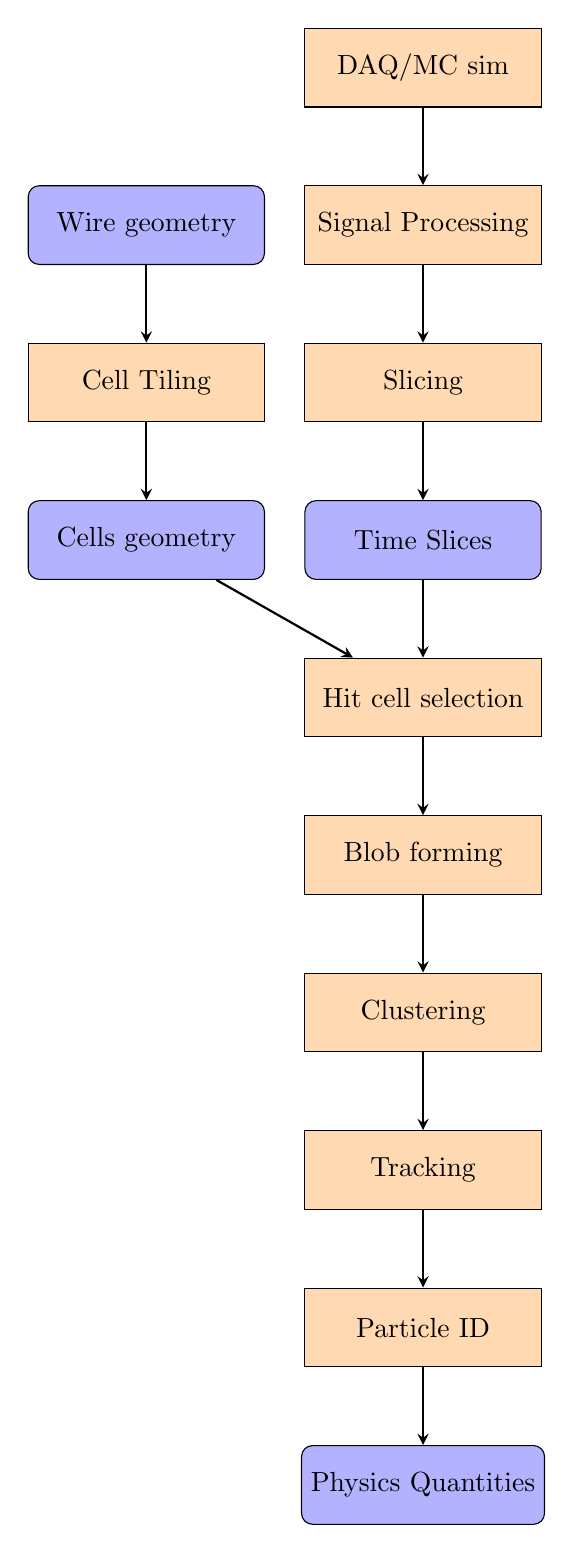
\begin{tikzpicture}[align=center, node distance=2cm]

\tikzstyle{dataobj} = [rectangle, rounded corners, minimum width=3cm, minimum height=1cm,text centered, draw=black, fill=blue!30]
\tikzstyle{process} = [rectangle, minimum width=3cm, minimum height=1cm, text centered, draw=black, fill=orange!30]
\tikzstyle{decision} = [diamond, minimum width=3cm, minimum height=1cm, text centered, draw=black, fill=green!30]
\tikzstyle{arrow} = [thick,->,>=stealth]

\node (daqmc) [process,highlight=2] {DAQ/MC sim};
\node (frames) [process,highlight=2, below of=daqmc] {Signal Processing};
\node (slicing) [process,highlight=2, below of=frames] {Slicing};
\node (slices) [dataobj, below of=slicing] {Time Slices};
\node (wires) [dataobj, left=0.5cm of frames] {Wire geometry};
\node (tiling) [process,highlight=2, left=0.5cm of slicing] {Cell Tiling};
\node (cells) [dataobj, left=0.5cm of slices] {Cells geometry};
\node (hitcells) [process,highlight=3, below of=slices] {Hit cell selection};
\node (blobbing) [process,highlight=3, below of=hitcells] {Blob forming};
\node (clustering) [process,highlight=4, below of=blobbing] {Clustering};
\node (tracking) [process,highlight=4, below of=clustering] {Tracking};
\node (pid) [process,highlight=5, below of=tracking] {Particle ID};
\node (physics) [dataobj, below of=pid] {Physics Quantities};

\draw [arrow] (wires) -- (tiling);
\draw [arrow] (tiling) -- (cells);
\draw [arrow] (cells) -- (hitcells);
\draw [arrow] (daqmc) -- (frames);
\draw [arrow] (frames) -- (slicing);
\draw [arrow] (slicing) -- (slices);
\draw [arrow] (slices) -- (hitcells);
\draw [arrow] (hitcells) -- (blobbing);
\draw [arrow] (blobbing) -- (clustering);
\draw [arrow] (clustering) -- (tracking);
\draw [arrow] (tracking) -- (pid);
\draw [arrow] (pid) -- (physics);
\end{tikzpicture}}
      \end{center}
    \end{column}
  \end{columns}

\end{frame}

\subsection{Data Preparation}

\begin{frame}
  \frametitle{Framing}
  
  \vspace{-2.0cm}
  \begin{center}
    \rotatebox{-90}{\includegraphics[width=6cm]{framing.pdf}}    
  \end{center}
  \vspace{-1.0cm}

  \scriptsize
  Raw data stream readout in blocks or \textbf{frames} of time.

  Typical digitizing: $\sim$\SI{4}{\milli\second}, \SI{2}{\mega\hertz}, 12 bit/sample.

  \begin{columns}
    \begin{column}{0.5\textwidth}
      \scriptsize
      \textbf{MicroBooNE:}
      \begin{itemize}
      \item \textbf{Very active at surface}: $\sim$20 cosmic-$\mu$ events/frame.
      \item Very ``few'' channels (8256).
      \item \textbf{full-stream} readout frames, big but manageable:
        \textbf{$\sim$100 MB/frame}.
      \end{itemize}

    \end{column}
    \begin{column}{0.5\textwidth}
      \scriptsize
      
      \textbf{DUNE:}
      \begin{itemize}
      \item \textbf{Deep underground}, quiet detector.
      \item Isolated $^{39}$Ar decays dominant bkg.
      \item \textbf{1.5M channels} could produce: \\
        4.5 TB/second \textbf{full-stream}!
      \item DUNE must \textbf{zero-suppress} signals.
      \item \textbf{$\sim$2.5 MB/frame} (25 GB if no ZS!)
      \item requires \textbf{clever DAQ!}
      \end{itemize}

    \end{column}
  \end{columns}
\end{frame}

\begin{frame}[fragile]
  \frametitle{Time Slicing}
  
  \begin{columns}
    \begin{column}{0.35\textwidth}
      \begin{center}
        \vspace{-.5cm}

        \includegraphics[width=\textwidth]{slice.pdf}

        \vspace{-2cm}

        \includegraphics[width=\textwidth,trim=0cm 10cm 0cm 0cm,clip]{slice-3D.pdf}

        \scriptsize True hits.
      \end{center}
    \end{column}
    \begin{column}{0.6\textwidth}

      \includegraphics[width=\textwidth]{wires-and-true-hits.png}

      \begin{itemize} \scriptsize
      \item One \textbf{time slice} of the frame.
      \item Slice width is chosen to match electronics shaping time: 4
        FADC ``ticks'' = \SI{2}{\micro\second}.
      \item Identify selection of ``hit'' wires in the slice.
        \begin{itemize} \scriptsize
        \item[$\rightarrow$] hit = FADC charge above some threshold.
        \end{itemize}
      \end{itemize}
    \end{column}
  \end{columns}

\end{frame}

\subsection{Imaging Of Activity}

\begin{frame}[fragile]
  \frametitle{Tiling}

  \begin{center}
    \includegraphics[width=0.7\textwidth,trim=8.6cm 9cm 8.6cm 9cm,clip]{test_boundcells.pdf}

    Zoom in on the wires and their associated cells.
  \end{center}



  \footnotesize
  \begin{itemize}
  \item Associate a 2D ``cell'' with small region near every
    triple-crossing of one wire from each plane.
  \item Cells completely tile the plane, no gaps, no overlaps.
  \item Cell shapes and sizes depend on wire plane pitches, angles and
    offsets.
  \end{itemize}

  \textbf{The heart of the Wire Cell concept:} if all three
  triple-crossing wires are ``hit'', the associated cell likely
  contains drifted charge.

\end{frame}

\begin{frame}
  \frametitle{Cell Ambiguity - Example Hit Pattern}

  \begin{columns}
    \begin{column}{0.5\textwidth}
      \includegraphics[width=\textwidth,trim=1cm 4cm 2cm 1cm,clip]{example-hit-cells.pdf}
    \end{column}
    \begin{column}{0.5\textwidth}
      Ambiguity arises due to spatial multiplexing.
      \begin{description}\scriptsize
      \item[Good] wire v3 measures no charge, all its cells must be unhit.
      \item[Bad] surrounding hits induce ``ghost'' at \textbf{c4}.
      \item[Ambiguous] multiple cells measured by same wire.
      \end{description}
      In some cases ambiguity can not be resolved at the cell level.
    \end{column}
  \end{columns}
\end{frame}

\begin{frame}[fragile]
  \frametitle{Some Formalism}
  Expected charge measured on \textbf{wires} ($\vec{w}$) can be calculated
  knowing charge in \textbf{cells} ($\vec{c}$):

  \[\vec{w} = \mathbf{G_{wc}}\vec{c}\]

  $\mathbf{G_{wc}}$ is the wire/cell \textit{adjacency matrix}, purely
  geometrical and perfectly known, function of detector design.
  
  \begin{columns}
    \begin{column}{0.45\textwidth}
      \vspace{-5mm}

      \flushright \includegraphics[width=0.8\textwidth,trim=1cm 11cm 2cm 2cm,clip]{example-hit-cells.pdf}

    \end{column}
    \begin{column}{0.10\textwidth}
      $\Leftrightarrow$
    \end{column}
    \begin{column}{0.45\textwidth}

  \resizebox{0.7\textwidth}{!}{
    $\left(
      \begin{array}[h]{c}
        0.0\\
        1.0\\
        2.0\\
        2.0\\
        0.0\\

        1.0\\
        1.0\\
        0.0\\
        2.0\\
        1.0\\

        1.0\\
        2.0\\
        2.0\\
      \end{array}
    \right)
    = \left(
      \begin{array}[h]{ccccccccc}
        1&0&0&0&0&0&0&0&0\\
        0&1&0&1&0&0&0&0&0\\
        0&0&1&0&1&0&1&0&0\\
        0&0&0&0&0&1&0&1&0\\
        0&0&0&0&0&0&0&0&1\\

        0&0&0&0&0&0&1&0&0\\
        0&0&0&1&0&0&0&1&0\\
        1&0&0&0&1&0&1&0&0\\
        0&1&0&0&0&1&0&0&0\\
        0&0&1&0&0&0&0&0&0\\
        
        1&0&0&1&0&0&1&0&0\\
        0&1&0&0&1&0&0&1&0\\
        0&0&1&0&0&1&0&0&1\\
      \end{array}
    \right)
    \left(
      \begin{array}[h]{c}
        0.0\\
        1.0\\
        1.0\\
        0.0\\
        0.0\\
        1.0\\
        1.0\\
        1.0\\
        0.0\\
      \end{array}
    \right)$}
      
    \end{column}
  \end{columns}


  Wish to solve inverse: $\vec{c} = \mathbf{G_{wc}}^{-1}\vec{w}$.
  However, $N_{cells} \approx N_{wires}^2$ \\
  $\Rightarrow$ as $N_{cells}$ grows, more unknowns ($\vec{c}$) than knowns ($\vec{w}$)!
\end{frame}

\begin{frame}
  \frametitle{Form Blobs}
  \vspace{-10mm}
  \begin{columns}
    \begin{column}{0.5\textwidth}
      Goal: \textbf{reduce matrix size} and \textbf{remove ambiguity}.
    \end{column}
    \begin{column}{0.5\textwidth}
      \includegraphics[width=0.8\textwidth]{wires-and-true-hits.png}          
    \end{column}
  \end{columns}
      
  \begin{enumerate}
  \item Select all cells with all three wires ``hit''.
  \item Partition into spatially contiguous subsets: ``\textbf{blobs}''.
  \end{enumerate}
  Equation to solve is now:
  \[\vec{w_b} = \mathbf{G_{wb}} \vec{b}\]

  \begin{description}
  \item[$\vec{c} \to \vec{b}$] vector of charge in each blob.
  \item[$\mathbf{G_{wc}} \to \mathbf{G_{wb}}$] the wire-blob adjacency matrix for the slice.
  \item[$\vec{w} \to \vec{w_b}$] vector of charge on all wires associated with blob.
  \end{description}

\end{frame}

% maybe remove this slide...
\begin{frame}
  \frametitle{Another wrinkle: charge uncertainty}

  Measures of the drifting charge by a wire has uncertainty.
  \begin{itemize}
  \item Noise from electronics and thermal fluctuations.
  \item Statistical uncertainty due to digitization.
  \item Systematic uncertainties from detector response deconvolution.
  \item Can be correlated across wires.
  \end{itemize}
  Compare measured wire charge ($\vec{w}_{meas}$) with expected
  ($\vec{w}_{exp}$) and form a $\chi^2$ with $\mathrm{V}$ a
  covariance uncertainty matrix.
  
  \[\chi^2 = (\vec{w}_{meas}-\vec{w}_{exp})^\intercal\mathrm{V}^{-1} (\vec{w}_{meas}-\vec{w}_{exp})\]

  ``It can be shown'' that minimizing this $\chi^2$ is equivalent to
  inverting $\mathbf{G_{wc}}$ (or $\mathbf{G_{wb}}$) matrix equation.

\end{frame}

\begin{frame}[fragile]
  \frametitle{The Payoff: imaged \SI{3}{\giga\electronvolt} $\nu_e$ interaction}
  
  \begin{columns}
    \begin{column}{0.5\textwidth}
      \begin{center}
        \includegraphics[width=\textwidth]{payoff-true.png}

        True energy depositions.
      \end{center}
    \end{column}
    \begin{column}{0.5\textwidth}
      \begin{center}
        \includegraphics[width=\textwidth]{payoff-reco.png}

        Blob-level reconstruction.
      \end{center}
    \end{column}
  \end{columns}
\end{frame}


\subsection{Pattern Recognition}

\begin{frame}
  \frametitle{Clustering, Tracking and Categorization}
  Post-imaging, current approach:
  \begin{enumerate}
  \item \textbf{cluster} together blobs contiguous in space and time
    (slice).
  \item \textbf{track} a line through a cluster.
  \item \textbf{categorize} success/failure of line to account for the
    cluster's charge distribution.
  \end{enumerate}
  Some categories:
  \begin{description}
  \item[track] cluster is well fit by the track
  \item[short] cluster appears to be a ``short track'' (eg, $\delta$-ray)
  \item[shower] cluster appears to be a EM/hadronic shower
  \item[undefined] no well-suited categorization.
  \end{description}

  This is an active area of development.

\end{frame}

\subsection{Physics}
\begin{frame}
  \frametitle{Physics-level Reconstruction}

  This development is just beginning.
  
  It will:
  \begin{itemize}
  \item associate clusters with a particle trajectory
  \item determine particle type
  \item determine momentum, range, dE/dx and other kinematics.
  \end{itemize}

\end{frame}


\section{Software Design}

\begin{frame}
  \tableofcontents[currentsection,hideothersubsections]
\end{frame}

\subsection{Software Overview}

\begin{frame}
  \frametitle{Wire Cell Software Ecosystem}

  Wire Cell breaks up into three main parts:

  \begin{description}
  \item[visualization] the ``Bee'' web application (Chao Zhang)
  \item[prototype] reconstruction algorithms, initial proof of
    principle (Xin Qian)
  \item[toolkit] production toolkit (bv)
  \end{description}

\end{frame}

\subsection{Bee Display}

\begin{frame}
  \frametitle{Bee Features}

  Bee is a 3D interactive visualization system:
  \begin{itemize}
  \item Displays results of different reconstruction algorithms.
  \item Shows ``true'' particle trajectories from simulation.
  \item Very good for developers to compare and debug and users to
    gain Physics intuition.
  \item Implemented as JavaScript/WebGL front-end and Django back-end.
  \item Works on popular desktop and mobile browsers.
  \item Requires hardware WebGL support.
  \item JSON data file format, easy to implement schema.
  \item Supports drag-and-drop
    \href{http://bnlif.github.io/wire-cell-docs/viz/uploads/}{user
      file uploads}.
  \item New features almost daily (\textbf{Chao Zhang}!)
  \end{itemize}
\end{frame}

\begin{frame}
  \frametitle{Bee: Select and upload event sets}
  \begin{center}
    \includegraphics[height=0.8\textheight]{bee-event-sets-page.png}    
  \end{center}
\end{frame}
\begin{frame}
  \frametitle{Interactive 3D visualization}
  \begin{center}
    \includegraphics[height=0.8\textheight]{bee-full-gui.png}    
  \end{center}
\end{frame}

\begin{frame}
  \frametitle{Bee: Online Demo}
  \begin{center}
    \url{http://www.phy.bnl.gov/wire-cell/bee/}
  \end{center}
\end{frame}

\subsection{Prototype}

\begin{frame}
  \frametitle{Wire Cell Working Prototype}
  \footnotesize
  The prototype:
  \begin{itemize}
  \item \textbf{Very successful proof of principle!}
  \item Currently \textbf{leads the state of the art} in LArTPC
    reconstruction techniques.
  \item Amazingly fast development (\textbf{Xin Qian}!)
  \end{itemize}
  Some compromises:
  \begin{itemize}
  \item Avoid support for long-term, multi-developer contributions.
  \item Many monolithic, single-threaded applications.
  \item Some hard-coded ``magic'' numbers, lack of configuration.
  \item Rigid code structure, hard-coded workflows.
  \item Integrate with external frameworks via exchange files.
  \item Some spot CPU/memory optimization, expect more improvement.
  \item Some high-level tests but lack of granular coverage.
  \item Intimate dependency on ROOT\footnote{\url{https://root.cern.ch/}}.
  \end{itemize}
  
  The ``production'' toolkit attempts to address these issues
\end{frame}

\subsection{Toolkit}

\begin{frame}
  \frametitle{Wire Cell Toolkit}
      
  \begin{columns}
    \begin{column}{0.6\paperwidth}
    \end{column}
    \begin{column}{0.4\paperwidth}
      \vspace{-20mm}
      \includegraphics[width=\textwidth]{deps.pdf}      
    \end{column}
  \end{columns}

  \vspace{-10mm}

  High level overview:
  \begin{itemize}
  \item Software \textbf{packaging and build} system.
  \item Comprehensive \textbf{API} via abstract base classes.
  \item Wire and cell \textbf{geometry} descriptions.
  \item Simple LArTPC detector \textbf{simulation}.
  \item Refactored implementation of \textbf{prototype algorithms}.
  \item Abstracted \textbf{execution model}.
  \item Support for internal and external \textbf{file I/O}.
  \end{itemize}

\end{frame}

\begin{frame}[fragile]
  \frametitle{Source Repositories and Build}

  \begin{itemize}
  \item Code in GitHub \href{https://github.com/WireCell/}{WireCell} organization.
  \item Code aggregation with \textbf{git submodule}.
  \item A simple, customized \href{https://waf.io/}{waf}-based build.
  \end{itemize}

  \begin{lstlisting}{langauge=shell}
$ git clone git@github.com:WireCell/wire-cell.git
$ cd wire-cell/
$ git submodule init
$ git submodule update
$ ./wcb --prefix=/path/to/install configure build install
  \end{lstlisting}
%$

  Builds, tests and installs:
  \begin{itemize}
  \item shared libraries + header files,
  \item main applications,
  \item many unit tests,
  \item \href{http://www.phy.bnl.gov/wire-cell/doxy/html/}{Doxygen reference} and \href{http://wirecell.github.io/wire-cell-docs/}{MkDocs user documentation}.
  \end{itemize}

  \scriptsize Note: \texttt{wcb} = \texttt{waf} + extra Waf tools for Boost, ROOT, Eigen
  and Wire Cell packaging
  

\end{frame}

\begin{frame}[fragile]
  \frametitle{Wire Cell Interfaces}

  The \href{https://github.com/WireCell/wire-cell-iface}{\texttt{wire-cell-iface}} package:

  \begin{itemize}
  \item Comprehensive detailed API
    \begin{itemize}
    \item Data model (wires, cells, frames, slices, tracks, ...)
    \item Active components (blob maker, matrix solver, clutering, ...)
    \end{itemize}
  \item Use of C++ \verb|shared_ptr<>| memory management.
  \item Dynamic instance lookup via \texttt{NamedFactory} pattern
    allows for a plugin architecture.
  \item Initial support for user configuration system based on Boost
    property trees.
  \item Initial abstract execution model (more on this)
  \end{itemize}
\end{frame}

\begin{frame}
  \frametitle{Wire Cell Simulation}

  The \href{https://github.com/WireCell/wire-cell-gen}{\texttt{wire-cell-gen}} package:
  \begin{itemize}
  \item Simple and granular implementation of the 4 LArTPC D's:
    deposit, drift, diffuse, digitize.
  \item Reference implementation for external frameworks to start from.
  \item Test bed for Wire Cell 
    architectural/toolkit concepts
  \item Provides on-the-fly generated input data for unit tests.
  \end{itemize}


\end{frame}

\begin{frame}[fragile]
  \frametitle{Wire Cell Execution Model}

  \begin{columns}
    \begin{column}{0.7\textwidth}
      \footnotesize 
      The toolkit supports \textit{data flow programming} paradigm
      \begin{itemize}
        \item Directly influenced by \href{http://www0.bnl.gov/events/details.php?q=8932}{CSC Seminar on VisTrails, March 2013}!
        \item Data flows through a graph made from:
          \begin{description}
          \item[vertices] computational units / algorithms
          \item[edges] data queues of a given type
          \end{description}
        \item Vtx has well defined input/output data types.
        \item Edges can be thread-safe queues.
        \item Graph-level programming.
        \item Can minimize necessary data buffering.
        \item Graph machinery replaceable: uniproc, multiproc, or
          distributed (MPI) parallel.
        \item Encourages isolated, targeted development and testing of each
          compute vertex.
        \end{itemize}
      \end{column}
      \begin{column}{0.3\textwidth}

        \vspace{-10mm}

        \includegraphics[width=\textwidth]{dataflow.pdf}
      \end{column}
    \end{columns}
\end{frame}

\begin{frame}
  \frametitle{Abstract execution model}
  Three layers for each graph vertex, outside to in:
  
  \begin{columns}
    \begin{column}{0.6\textwidth}
      \begin{enumerate}
      \item Execution model layer implementing data flow control
        (eg: sync'ed load-and-flush, async, multi-processing, ...)
      \item Adapter to abstract execution model client, calls actual algorithm.
      \item Algorithm implementation and interface unrestricted except ``no shared
        globals'' 
      \end{enumerate}
    \end{column}
    \begin{column}{0.4\textwidth}
      \includegraphics[width=1.1\textwidth]{concentric.pdf}      
    \end{column}
  \end{columns}

\end{frame}

\section{Future Plans}

\begin{frame}
  \tableofcontents[currentsection,hideothersubsections]
\end{frame}

\subsection{Bee 2.0}

\begin{frame}
  \frametitle{Current Limitations}
  Pattern recognition stage is turning out to be ``hard''(er!)
  \begin{itemize}
  \item The problem is largely independent of Wire Cell imaging techniques.
  \item Very large solution space with many corner cases.
  \item Humans excel at ad-hoc, high quality, Physics-driven solutions.  But, difficult to:
    \begin{itemize}
    \item estimate humans' systematic uncertainies and biases.
    \item enumerate and teach computers all these solutions.
    \item (impossible?) to teach computers to come up with
      solutions themselves.
    \end{itemize}
  \end{itemize}
  
  Probably entering an area of ``real'' computer science problems like machine learning.  

  And we are no experts!

\end{frame}

\begin{frame}
  \frametitle{Bee 2.0: Human-directed Automated Reconstruction}
  Interim Solution: inject human judgment to guide Wire Cell reconstruction.
  \begin{enumerate}
  \item Develop \textbf{Bee} to provide human-driven interactive control of reconstruction.
    \begin{itemize}
    \item ``Join Cluster X to Cluster Y''
    \item ``Remove Blob AAA from Cluster Z''
    \end{itemize}
  \item Convert human commands into operational objects.
  \item Send to back end, execute inside a Wire Cell service.
  \item Send results back to user.
  \item Record everything in a database to mine for potential Wire
    Cell improvements.
  \end{enumerate}
  Think: ``\textbf{Physics-PhotoShop}'' + ``\textbf{Google Analytics}''
\end{frame}

\begin{frame}
  \frametitle{Bee 2.0: Architecture}
  Interactive Wire Cell will likely include:
  \begin{itemize}
  \item Move Bee from Three.js to a new JS/WebGL framework to support interactive controls (eg ``picking'').
  \item Develop a web-friendly batch workflow system (probably based on Celery).
  \item Develop a database system to capture and control the system (likely to use MongoDB).
  \item Develop the Django back end into a middle-ware layer to tie this all together.
  \item Provision the hardware to support all this.
  \end{itemize}

  These are big plans and we are not experts in much of it.  

  \textbf{Help wanted!}

\end{frame}

\subsection{Parallel Wire Cell}

\begin{frame}
  \frametitle{Taking Wire Cell Parallel}
  Wire Cell is a 1-2 punch for today's computing:
  \begin{itemize}\footnotesize
  \item[$\rightarrow$] Needs high thoughput to keep up with detector data rates.
  \item[$\rightarrow$] Needs high performance due to CPU-heavy algorithms.
  \end{itemize}
  Plans, roughly in order:
  \begin{enumerate}\footnotesize
  \item Exec. model for \href{https://github.com/erenon/pipeline}{Boost.Pipeline} nice, simple threaded data flow package, but experimental (not officially part of BOOST)
  \item Exec. model for \href{https://www.threadingbuildingblocks.org/}{Intel TBB} a common and well supported library with a fantastic looking ``flow graph designer'' tool.
  \item Exec. model for MPI or other ways to run Wire Cell as multi-node (eg \textbf{HPC}) distributed process.
  \item Investigate potential for \textbf{GPU/Phi} hardware acceleration.
  \end{enumerate}

  This level of parallelism is new to us (and to much of HEP in general) and is a subject of a pending LDRD proposal.

  \textbf{Help wanted!}
\end{frame}

\subsection{Algorithm Development}

\begin{frame}
  \frametitle{}
  
  
  
  
\end{frame}

\section{}

\begin{frame}
  \frametitle{Summary}
  \begin{itemize}
  \item The \textbf{Wire Cell working prototype LArTPC reconstruction} method and software has been developed.
    \begin{itemize}
    \item producing some of the best results,
    \item much improvement still needed.
    \end{itemize}
  \item The \textbf{Bee interactive 3D event visualization} application has been developed.
  \item The \textbf{Wire Cell Toolkit} for long term development and support of
    parallel processing has been developed.
  \item Many areas at different levels are still in development.
  \item We find that to be successful we are going into \textbf{new waters}
    (for us) of massive parallel processing, hardware acceleration,
    computing science and mathematics.
    \begin{itemize}
    \item[$\rightarrow$] \textbf{Expert input, help and collaboration is most welcome!}
    \end{itemize}
  \end{itemize}
\end{frame}

\begin{frame}
  \frametitle{Wire Cell on the web}

  \begin{itemize}
  \item home page: \\ \url{http://www.phy.bnl.gov/wire-cell/}
  \item Bee entry: \\ \url{http://www.phy.bnl.gov/wire-cell/bee/}
  \item prototype user manual: \\ \url{http://bnlif.github.io/wire-cell-docs/}
  \item toolkit user manual: \\ \url{http://wirecell.github.io/wire-cell-docs/}
  \item toolkit reference: \\ \url{http://www.phy.bnl.gov/wire-cell/doxy/html/}
  \item prototype repositories: \\ \url{https://github.com/BNLIF}
  \item toolkit repositories: \\ \url{https://github.com/WireCell}
  \end{itemize}
\end{frame}

\end{document}


%%% Local Variables:
%%% mode: latex
%%% TeX-master: t
%%% End:
